\documentclass[preprint]{rmxac}


%%%
%%% Define any personal macros here
%%% 

% These are some I use in typesetting example code
\newcommand{\bs}{\textbackslash}
\newcommand{\CS}[1]{\texttt{\textbackslash #1}}
% roman subscripts in math
\newcommand{\Sub}[1]{_\mathrm{#1}}
% a command to specify possible linebreak points in an email address 
\newcommand{\D}{\discretionary{}{}{}}

%%%
%%% Article preamble commands (title, authors, abstract, etc.) 
%%% None of these produce any output themselves, they just set things 
%%% up for \maketitle
%%%

% This is only used for making the header for the preprint version
\SetYear{2007}
\SetConfTitle{Name of Conference}

% Please use mixed case here, since this title gets propagated onto
% the web page, ADS entry, etc. 
\title{A Demonstration One-Page Contribution for the RevMexAA Conference Series}

\author{
  W. J. Henney\altaffilmark{1,2,3}}


% Note that \altaffil, \altaffilmark go inside the scope of the
% \author{...} command but \altaffiltext is outside it. 
\altaffiltext{1}{Centro de Radioastronom\'\i{}a y Astrof\'\i{}sica,
  Universidad Nacional Aut\'o\-noma de M\'e\-xico, Apartado Postal
  3--72, 58090 Morelia, Michoac\'an, M\'exico
  (w.henney\D{}@astrosmo.\D{}unam.\D{}mx).}
\altaffiltext{2}{Please note that affiliations end in periods.}
\altaffiltext{3}{The full postal
  addresses should go here. However, if there are many authors and
  space is short, then just the full address of the first author will
  do.}

% The following is necessary to tell the macros not to try and typeset
% the full addresses at the end of the article
\suppressfulladdresses

% List of authors used to construct table of contents
\listofauthors{W. J. Henney}
% Each author in Surname, Initials format, used in generating Author
% Index entries.
\indexauthor{Henney, W. J.}

% No \abstract or \resumen for poster papers

% Keywords must be from the standard list and in alphabetical order. 
\addkeyword{H~II regions}
\addkeyword{ISM: Jets and outflows}
\addkeyword{Stars: Pre-main sequence}
\addkeyword{Stars: Mass loss}

%%%
%%% Beginning of document proper
%%%
\begin{document}
% Typeset article header
\maketitle 

\boldabstract{This document (\texttt{rm-onepage.tex}---last updated
  2007 Sep 9) can serve as a template for the preparation of one-page
  conference proceedings contributions with the \texttt{rmaa} \LaTeX{}
  macros. Note that the standard abstract environment is \emph{not}
  used and there is no Spanish resumen.}


Given that you only have one page, you probably don't want to waste
space with frivolities such as section headings.  

The general structure of the flow variables along the symmetry axis of
the bowshock shell is illustrated schematically in
Figure~\ref{fig:simple}.  The approximately isothermal proplyd flow
accelerates from the sound speed up to a Mach number $\mathcal{M}_0$
at the position of the shock. If the number density and temperature
immediately before the shock are $N_0$, $T_0$, then the
Rankine-Hugoniot conditions give the values immediately after
the shock to be (Landau \& Lifschitz 1987)
\begin{equation}
  \label{eq:mjump}
  \mathcal{M}_1 = \left( \frac{ \mathcal{M}_0^2 + 3 } { 5
      \mathcal{M}_0^2 - 1 } \right)^{1/2} , 
\end{equation}
\begin{equation}
  \label{eq:njump}
  N_1 = \frac{ 4 } { 1 + 3 \mathcal{M}_0^{-2} } N_0 , 
\end{equation}
\begin{equation}
  \label{eq:tjump}
  T_1 = \frac{1}{16} \left( 5 \mathcal{M}_0^2 - 1 \right) 
  \left( 1 + 3 \mathcal{M}_0^{-2} \right) T_0 .
\end{equation}
For instance, using $\mathcal{M}_0 = \mathcal{M}\Sub{A} = 2.7$ from
equation~(99), one obtains $\mathcal{M}_1 = 0.54$,
$N_1 = 2.83 N_0 = 5.77 \times 10^4$\,cm$^{-3}$, $T_1 = 3.13 T_0 =
30,500$\,K, so that the density and temperature jump across the shock
are both roughly a factor of 3.

The emission from the cooling zone behind the shock can be crudely
approximated as the emission from a homogeneous layer with density
$N_1$ and temperature $T_1$ and with a width equal to the cooling time
$t\Sub{cool} = 3 k T_1 / \left( N_1 \Lambda_1 \right)$ multiplied by
the immediate post-shock velocity $v_1 = \mathcal{M}_1 (T_1/T_0)^{1/2}
c_0 \simeq 11.5$\,km\,s$^{-1}$. In order to estimate the cooling
coefficient $\Lambda_1$ in the cooling zone I calculated another
Cloudy model, identical to that mentioned above except that the
electron temperature was artificially maintained at $T\Sub{e} = T_1$.
The result was $\Lambda_1 = 4.46 \times
10^{-23}$\,erg\,cm$^{3}$\,s$^{-1}$, giving a cooling time $t\Sub{cool} =
4.9 \times 10^6$\,s and a cooling zone thickness $h\Sub{cool} = 5.64
\times 10^{12}$\,cm. Although the \ion{O}{3} optical lines are still
significant coolants in the cooling zone (20\% of total), they are now
supplanted in importance by the \ion{C}{3} NUV (28\%) and FUV (26\%)
lines.


\begin{figure}[!t]
  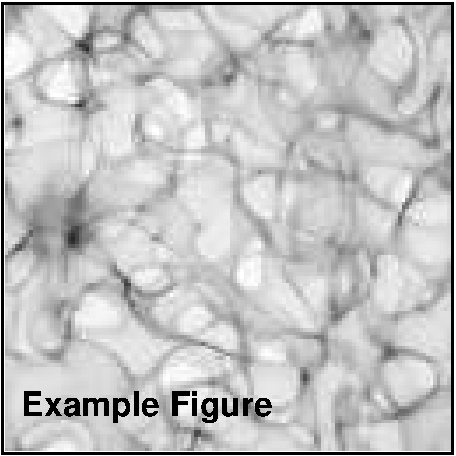
\includegraphics[width=\columnwidth]{example-fig}
  \caption{Example of a simple single-column figure. Don't put this
    too early in the document since we don't want it to go in the
    first column.}
  \label{fig:simple}
\end{figure}

\dots and that is all there is room for.

\begin{thebibliography}

\bibitem{Bal98} Bally, J., Sutherland, R.~S., Devine, D., \&
  Johnstone, D. 1998, AJ, 116, 293

\bibitem{Bate} Bate, M.~R., Clarke, C., \& McCaughrean, M.~J. 1998,
  MNRAS, 297, 1163

\bibitem{CRW} Cant\'o, J., Raga, A.~C., \& Wilkin, F.~P. 1996, ApJ,
  469, 729 (CRW)

\bibitem{Fulgencio} Garc\'\i a-Arredondo, F., Henney, W.~J., \& Arthur,
  S.~J. 2001, ApJ, 561, 830 
  
\end{thebibliography}

\end{document}
